\subsection{Navigation}
\label{cha:navigation}

The interactions that let users move between, inside, and outside of the various pieces of content in a app are referred to as navigation. The Navigation component of Android Jetpack assists in implementing navigation, from straightforward button clicks to more intricate patterns like app bars and the navigation drawer. The navigation component also ensures a consistent and predictable user experience by adhering to a set of principles \cite{android_navigation}.

The main navigation concept conists of three major parts:
\begin{itemize}
    \item NavController manages the navigation workflow. When a new destination should be visible, the NavController sends the UI elements to the NavHost. It also take care of the Back Stack when interacting with different destinations. When the user wants to go back, the NavController know exactly which destination was the previous one. The controller is read out as follows:
    
    \noindent
    \lstinline{val navController = rememberNavController()}
    
    \item NavHost is a container which displays the composable functions of the destinations. Here follows an example:
    
\begin{lstlisting}[language=Kotlin]
val start = "screen1"
NavHost(navController, start) {
    composable("screen1") {
        Screen1()
    }
    composable("screen2") {
        Screen2()
    }
}
\end{lstlisting}

    \item Navigation Graph: defines the possible ways to navigate through the application. Before Jetpack Compose this component was declared in a XML file, where the single destinations and the interactions between them can be defined. Like in this example \cite{Figure_3} you define a start destination and from there on you have 2 different possible ways to navigate through the application. You can go to the registration or view the leader board.
    
    \begin{figure}[ht]
        \centering
        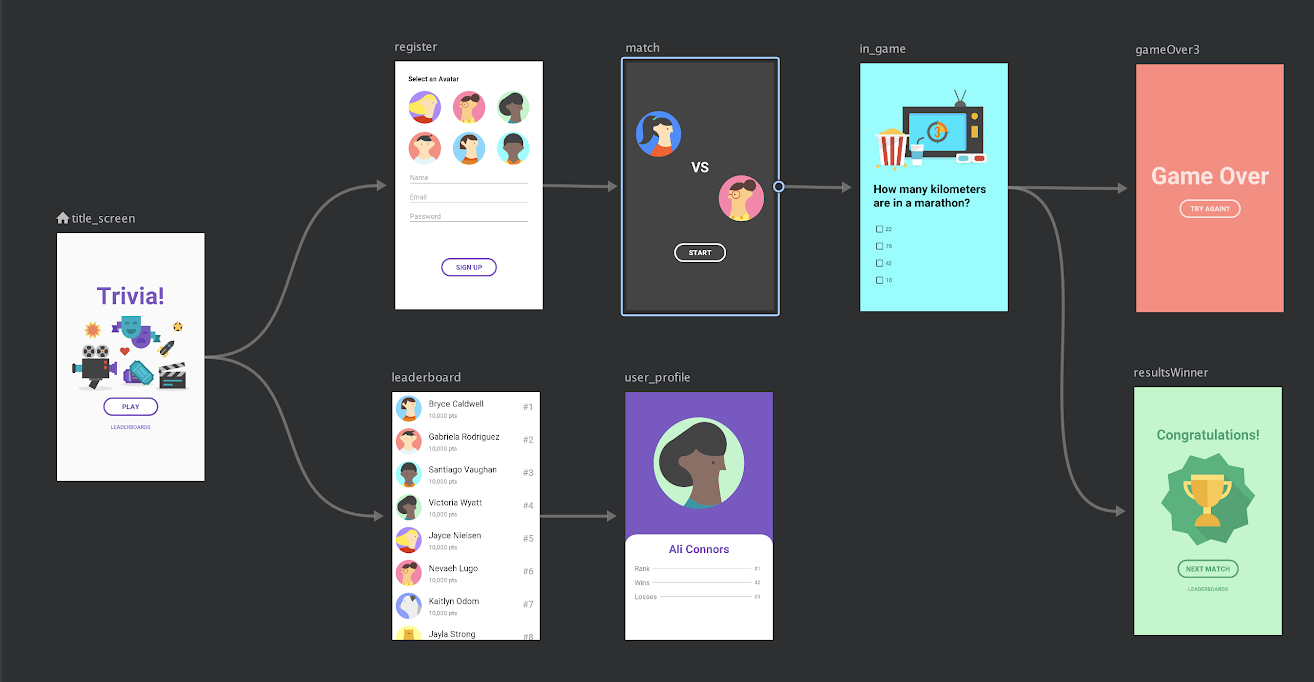
\includegraphics[width=\linewidth]{images/navigation_graph.png}
        \caption{Example navigation graph \cite{Figure_3}}
        \label{fig:navgraph}
    \end{figure}
    % https://miro.medium.com/max/1400/1*ESf1y0VYcHE5ldkCDD8HKA.png
    
\end{itemize}